\chapter{Analisi Sperimentale}
In questo capitolo verranno mostrati i risultati ottenuti applicando i due algoritmi descritti nei capitoli precedenti, Algoritmo \ref{algoritmo} e Algoritmo \ref{algoritmo2} (rispettivamente discussi nei capitoli \ref{cap 2} e \ref{cap:3}).\\
Quello che verrà portato all'attenzione sono le distribuzioni dei diversi $ k $-treelet nei differenti grafi $ G $ su cui sono state effettuate le sperimentazioni,si mostrerà come cambiano i tempi nell'applicazione dei due algoritmi ed inoltre su un singolo grafo verrà mostrata una stima di accuratezza dei risultati ottenuti rispetto a quelli effettivi calcolati per mezzo dell'algoritmo implementato in \cite{bressan2019motivo}.\\\
Per la sperimentazione sono stati utilizzati quattro differenti grafi mostrati nella tabella \ref{Tabella:grafo}, dove vi è anche una breve descrizione per ognuno.
Come si può notare i grafi hanno finalità differenti questo per permettere di vedere come la distribuzione dei treelet nei grafi varia a seconda dello scopo di ognuno di essi.\\
Per effettuare le sperimentazioni si è fatto uso di una macchina equipaggiata di 96GiB di memoria principale e con CPU X5687 Intel(R) Xeon(R) a 3.60GHz con 12 MB di cache su L3, usando la Virtual Machine di Java (JVM).\\
Come è stato anche detto nei precedenti capitoli, si è sfruttato in entrambe le implementazioni il MultiThreading e, nello specifico, durante queste sperimentazioni si sono utilizzati 4 thread in totale.
\\
\\
\begin{table}
	\begin{tabular}{|p{3cm}|p{7cm}|p{2cm}|p{2cm}| }
		 \hline
		\multicolumn{4}{|c|}{Lista dei Grafi} \\
		\hline
		Nome del grafo & Descrizione & Nodi & Archi\\
		\hline
		\hline
		Wikipedia talk (communication) network (WiKi-Talk) \cite{leskovec2010predicting} & Grafo non orientato che indica che l'utente A e l'utente B hanno apportato modifiche sulla pagina di discussione di Wikipedia l'uno dell'altro (cioè, l'utente A ha modificato la pagina di discussione dell'utente B e viceversa). & 92 K & 360K\\
		\hline
	YeastNet \cite{babu2012interaction} & Interazioni di passaggi complessi tra membrane e proteine in ``$ Saccharomyces \ \ cerevisiae $'', dando origine a una rete biologica (non diretta) & 5K & 50K\\
		\hline
		 road-luxembourg-osm \cite{bader2013graph} & Parte della rete stradale relativa alla città di Lussemburgo (non orientata) & 110K & 120K\\
		 \hline
		 soc-Slashdot0902 \cite{leskovec2009community} & Rete di interazioni sociali & 82K & 870K \\ 
		 \hline
	\end{tabular}
\caption{Tabella che descrive i diversi grafi usati nelle sperimentazioni}
\label{Tabella:grafo}
\end{table}

Per prima cosa verrà mostrata la distribuzione dei treelet nei grafi (Figure \ref{distr:1}.\ref{distr:2},\ref{distr:3} e \ref{distr:4}).
Nello specifico per i grafi Wiki-Talk, YeastNet e road-luxembourg-osm osserveremo la distribuzione dei treelet nella tabella per $ k = 8 $, verrà limitata la visualizzazione ai 15 treelet più frequenti.
Mentre per soc-Slashdot0902 osserveremo la distribuzione dei treelet per $ k=7 $, in questo caso verranno mostrati tutti poichè il numero totale è ristretto a 11.
Il valore scelto per $ k $, in entrambi i casi, non rappresenta il limite raggiunto dall'esecuzione di entrambi gli algoritmi, ma semplicemente è l'ultimo valore per cui vengono prodotti valori che non superassero il limite di rappresentazione.
Nei grafici riportati di seguito le ascisse rappresentano i differenti treelet, mentre le ordinate rappresentano le distribuzioni in percentuale.
\counterwithin*{figure}{chapter}
\renewcommand{\thefigure}{\arabic{figure}}
\begin{figure}[htbp]
	\centering
	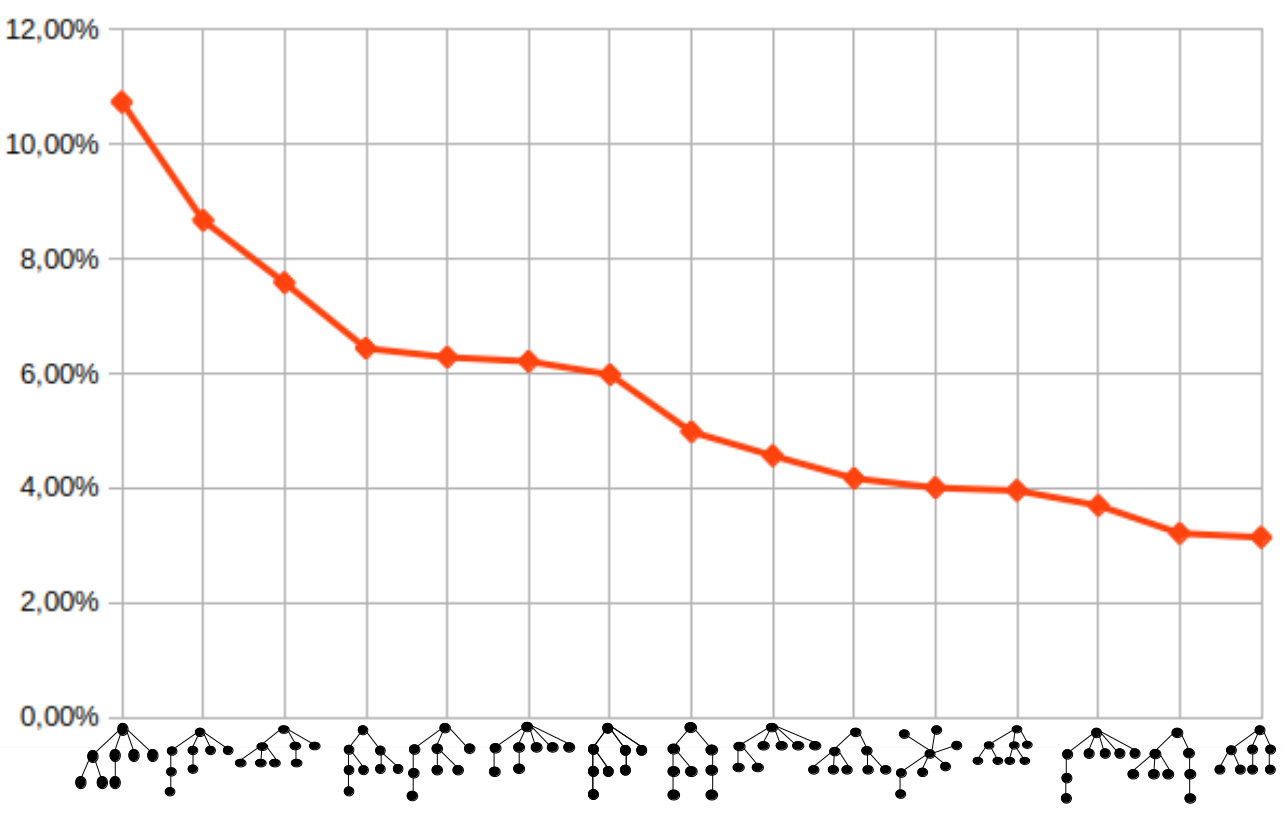
\includegraphics[width=15.4cm]{capitolo4/grafoWIKI}
		\caption{Distribuzione dei treelet con $ k=8 $ nel grafo WikiTalk}
		\label{distr:1}
\end{figure}\mbox{}
\\\\\\\\\\\\
\begin{figure}[htbp]
	\centering
	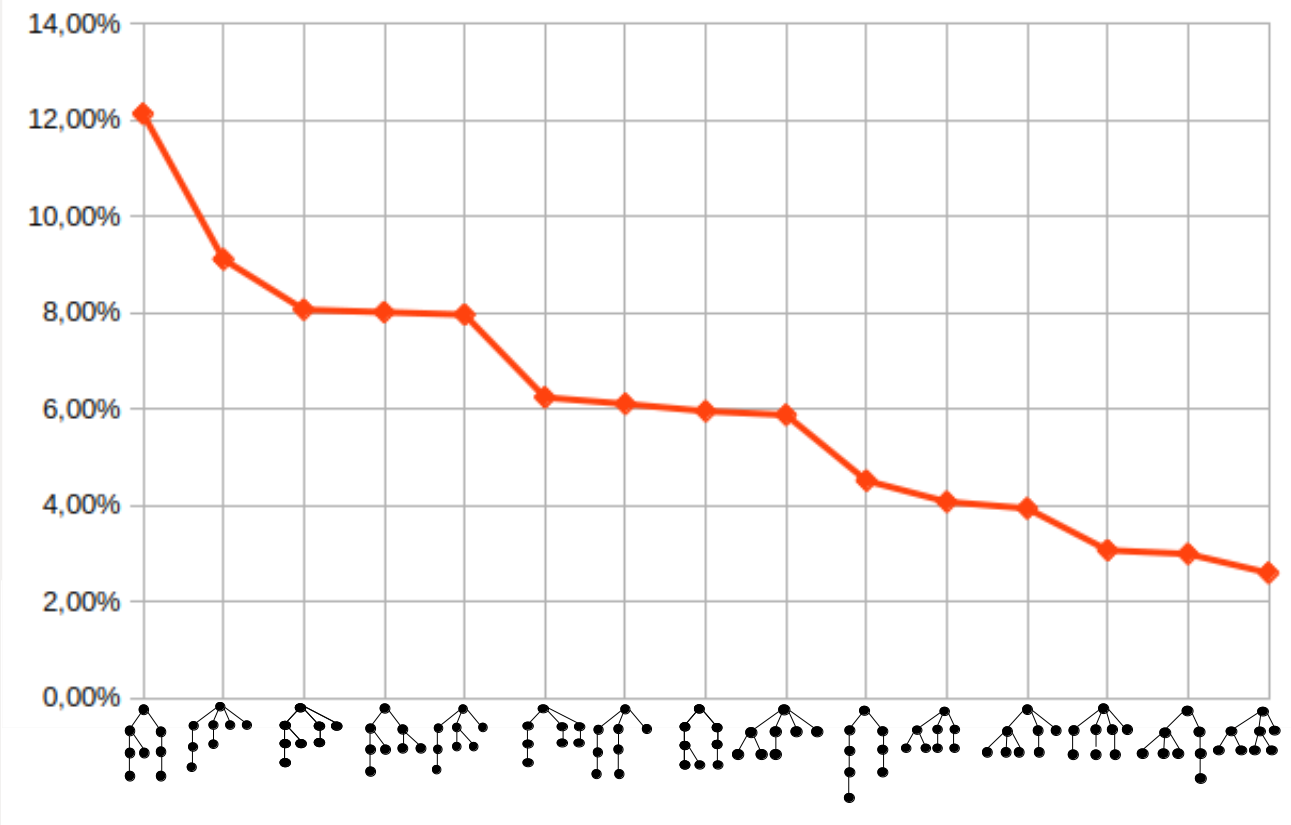
\includegraphics[width=15.4cm]{capitolo4/grafoYEAST}
	\caption{Distribuzione dei treelet con $ k=8 $ nel grafo YeastNet}
	\label{distr:2}
\end{figure}
\begin{figure}[htbp]
		\centering
	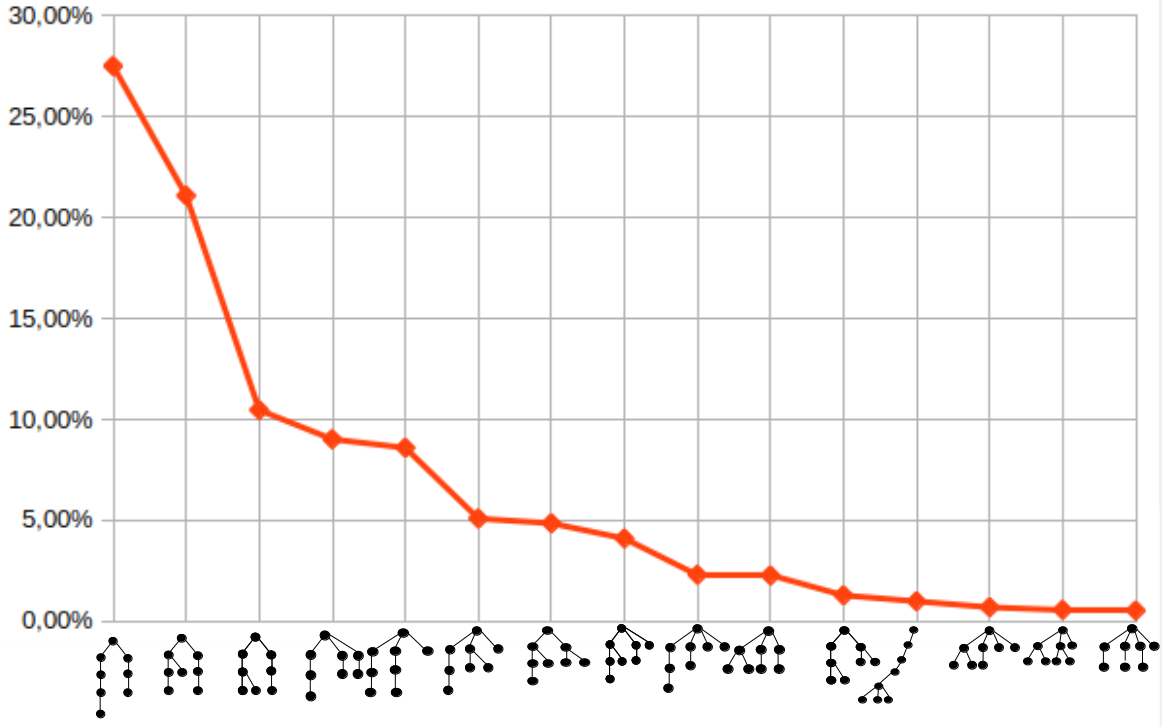
\includegraphics[width=15.4cm]{capitolo4/grafoROAD}	
		\caption{Distribuzione dei treelet con $ k=8 $ nel grafo road-luxembourg-osm }
		\label{distr:3}
\end{figure}
\begin{figure}[htbp]
		
	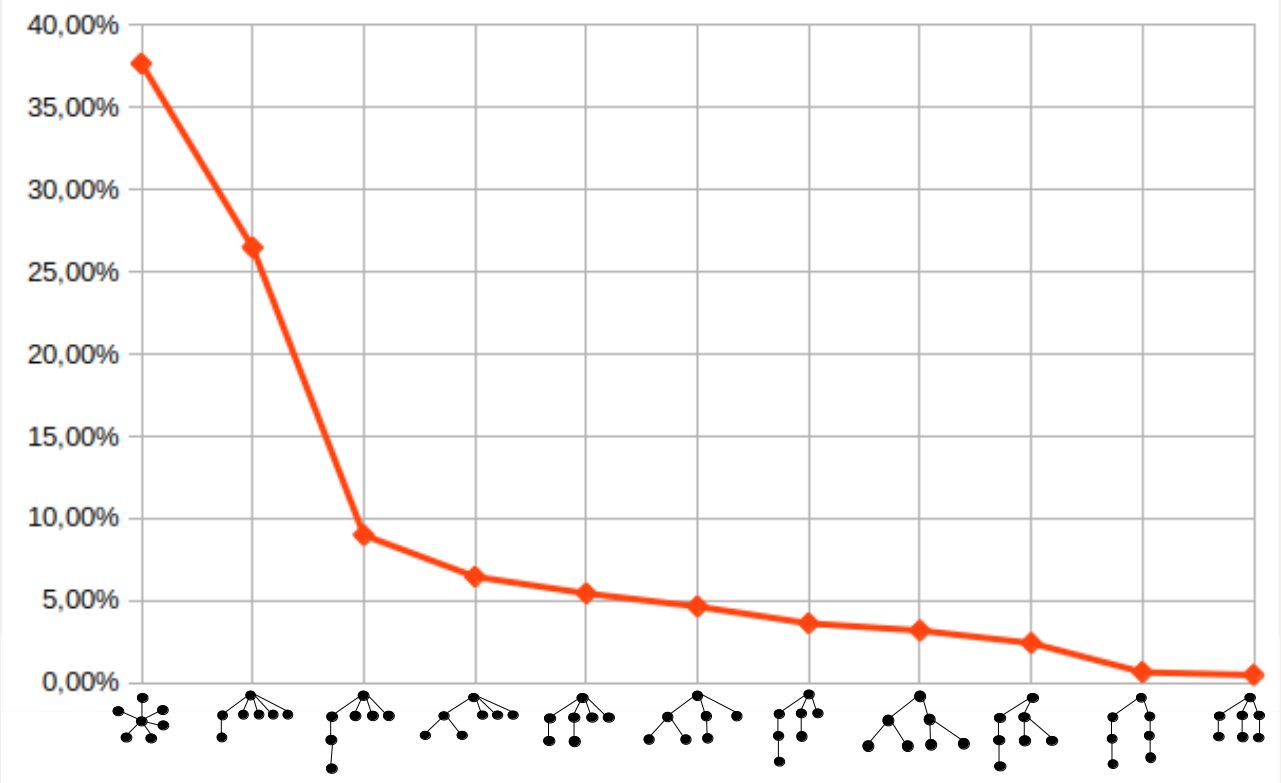
\includegraphics[width=15.4cm]{capitolo4/grafoALSH}
	\caption{Distribuzione dei treelet con $ k=7 $ nel grafo soc-Slashdot0902}
	\label{distr:4}
\end{figure}\mbox{}\\\\

Come si può notare analizzando velocemente i risultati nel grafo stradale (fig.\ref{distr:3}) e nel grafo sociale (fig.\ref{distr:4}) vi è una maggiore distribuzione di cammini e stelle, rispettivamente.
Mentre nel grafo biologico (fig.\ref{distr:2}) si possono notare strutture più complesse e maggiormente distribuite, così come nel grafo di figura \ref{distr:1}.

Un'altro aspetto interessante da vedere è come variano i tempi nell'utilizzo dei due algoritmi.
Nelle figure di seguito vengono mostrati, per ogni grafo e su ogni dimensione, tramite un istogramma, vengono messi a confronto i tempi di esecuzione delle due diverse implementazioni.

Come vedremo nelle figure \ref{Tempi:1},\ref{Tempi:2},\ref{Tempi:3}, l'asse delle ascisse rappresenta le diverse dimensioni dei treelet, ossia i diversi valori che $ k $ può assumere \ref{Tempi:4} le linee blu rappresentano i tempi relativi all'esecuzione dell'implementazione dell'Algoritmo \ref{algoritmo}, mentre le linee rosse indicano i tempi di esecuzione relative all'esecuzione dell'implementazione dell'Algoritmo \ref{algoritmo2}.
\\
\\

\begin{figure}[htbp]
	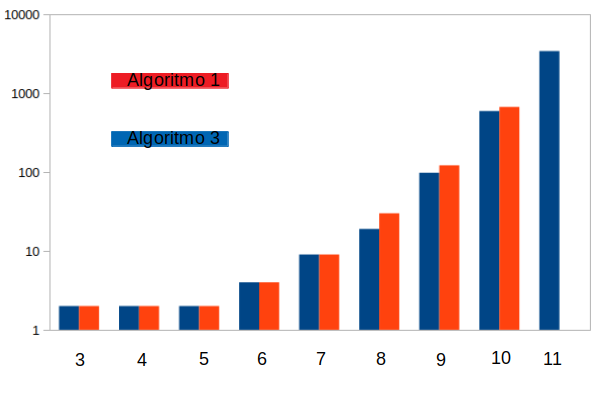
\includegraphics[width=15.4cm]{capitolo4/tempiWIKI}
	\caption{Tempi di esecuzione per gli Algoritmi \ref{algoritmo} e \ref{algoritmo2} sul grafo Wiki-Talk}
	\label{Tempi:1}
\end{figure}
\begin{figure}[htbp]
	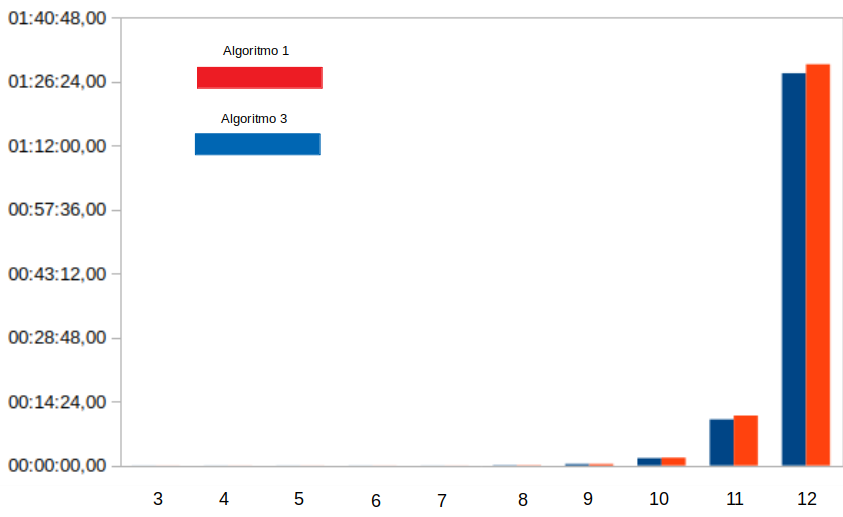
\includegraphics[width=15.4cm]{capitolo4/tempiYEAST}
	\caption{Tempi di esecuzione per gli Algoritmi \ref{algoritmo} e \ref{algoritmo2} sul grafo YeastNet}
	\label{Tempi:2}
\end{figure}
\begin{figure}[htbp]
	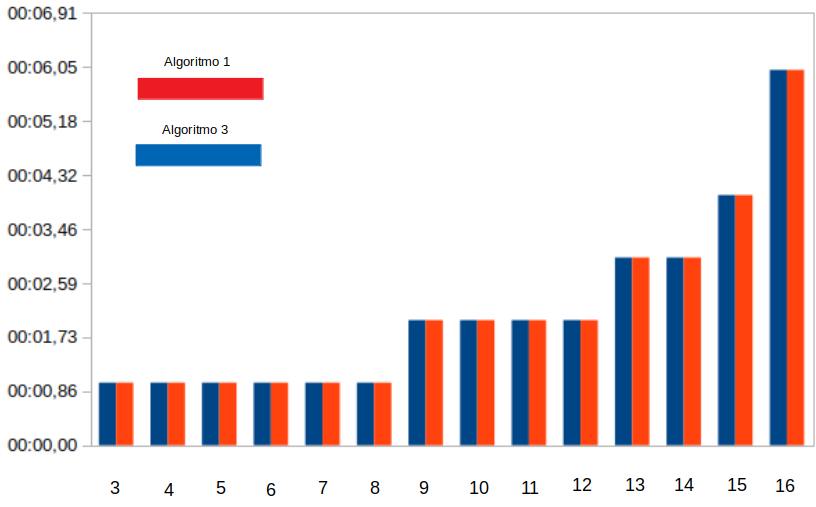
\includegraphics[width=15.4cm]{capitolo4/tempiROAD}
	\caption{Tempi di esecuzione per gli Algoritmi \ref{algoritmo} e \ref{algoritmo2} sul grafo road-luxembourg-osm}
	\label{Tempi:3}
\end{figure}
\begin{figure}[htbp]
	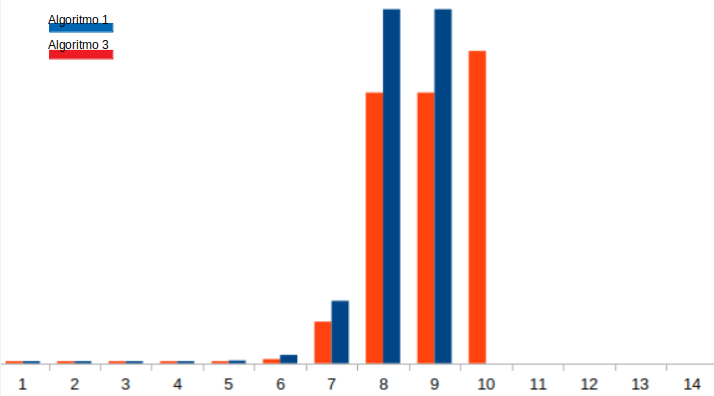
\includegraphics[width=15.4cm]{capitolo4/tempiSOC}
	\caption{Tempi di esecuzione per gli Algoritmi \ref{algoritmo} e \ref{algoritmo2} sul grafo soc-Slashdot0902}
	\label{Tempi:4}
\end{figure}

É facile notare come i tempi di esecuzione per l'implementazione ottimizzata siano minori rispetto a quella non ottimizzata.
L'unico grafo i cui tempi restano sostanzialmente in linea è quello biologico (fig.\ref{Tempi:2}), la causa principale da attribuirsi a ciò è la dimensione ridotta del grafo.
Infatti su grafi più grandi come ad esempio soc-Slashdot0902 (fig.\ref{Tempi:4}) la differenza si nota maggiormente. 
La scelta sulle dimensioni dei grafi, però, è stata vincolata dalla potenza della macchina a disposizione.
Ovviamente con grafi più grandi e con un maggior potenziale da sfruttare, si avrebbero avuto risultati più notevoli.
Un'altra cosa che si può notare vedendo i grafici, sono i differenti valori di $ k $ raggiunti.
Il motivo di ciò non è da attribuirsi al codice, bensì è stata una scelta forzata per risparmiare tempo.
Infatti ogni qualvolta l'esecuzione superava le due ore di tempo veniva interrotta, procedendo alla successiva.
Ed è proprio per questo motivo che per alcuni grafici, come ad esempio quello in figura \ref{Tempi:1} per $ k=8$ troviamo solo i tempi relativi al secondo algoritmo.
Per concludere l'analisi dei dati sperimentali ottenuti quello che si fa vedere ora è l'errore in norma $ \ell_1 $ rispetto al grafo YeastNet.
Quello che si vedrà è quanto i risultati reali si discostano dai risultati ottenuti in questa analisi.
Per calcolare $ \ell_1 $ si eseguono i seguenti cacoli. 
Sia $ f=(f_1,f_2,\dots,f_s) $ è il valore calcolato della frequenza dei $ k $-treelet in un grafo e sia $ \tilde{f}=(\tilde{f_1},\dots,\tilde{f_s}) $ lo stimatore, allora l'errore $ \ell_1 $ è $ \ell_1(f,\tilde{f}) = \sum_{i=1}^{s}{ (\tilde{f}-f)}$.
In questo caso calcolandolo per i valori di $ k $ da 3 a 9 sul grafo YeastNet potremo vedere che non supera mai l'1\% in tutti i casi.
Nel grafico \ref{ERROR} di seguito si può, vedere la linea dell'errore, sulle ascisse sono indicate le differenti dimensioni $ k $ mentre sulle ordinate si trovano le percentuali e si può chiaramente vedere come aumenta l'errore aumentando il valore di $ k $.   
\begin{figure}[htbp]
	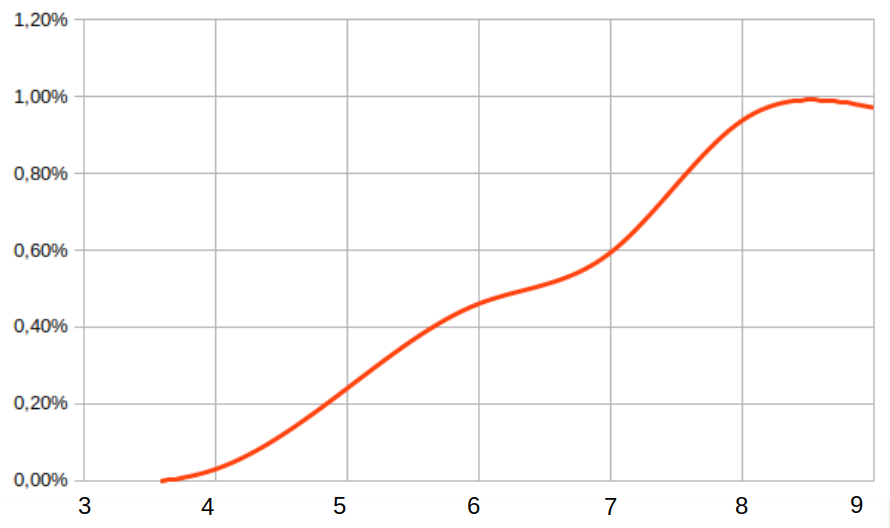
\includegraphics[width=15.4cm]{capitolo4/grafoErrorel1}
	\caption{Grafico dell'errore in norma $ \ell_1 $ sul grafo YeastNet, per dimensioni di $ k $ che variano da 3 a 9}
	\label{ERROR}
\end{figure}

